% Created by tikzDevice version 0.12.3.1 on 2022-09-02 16:25:13
% !TEX encoding = UTF-8 Unicode
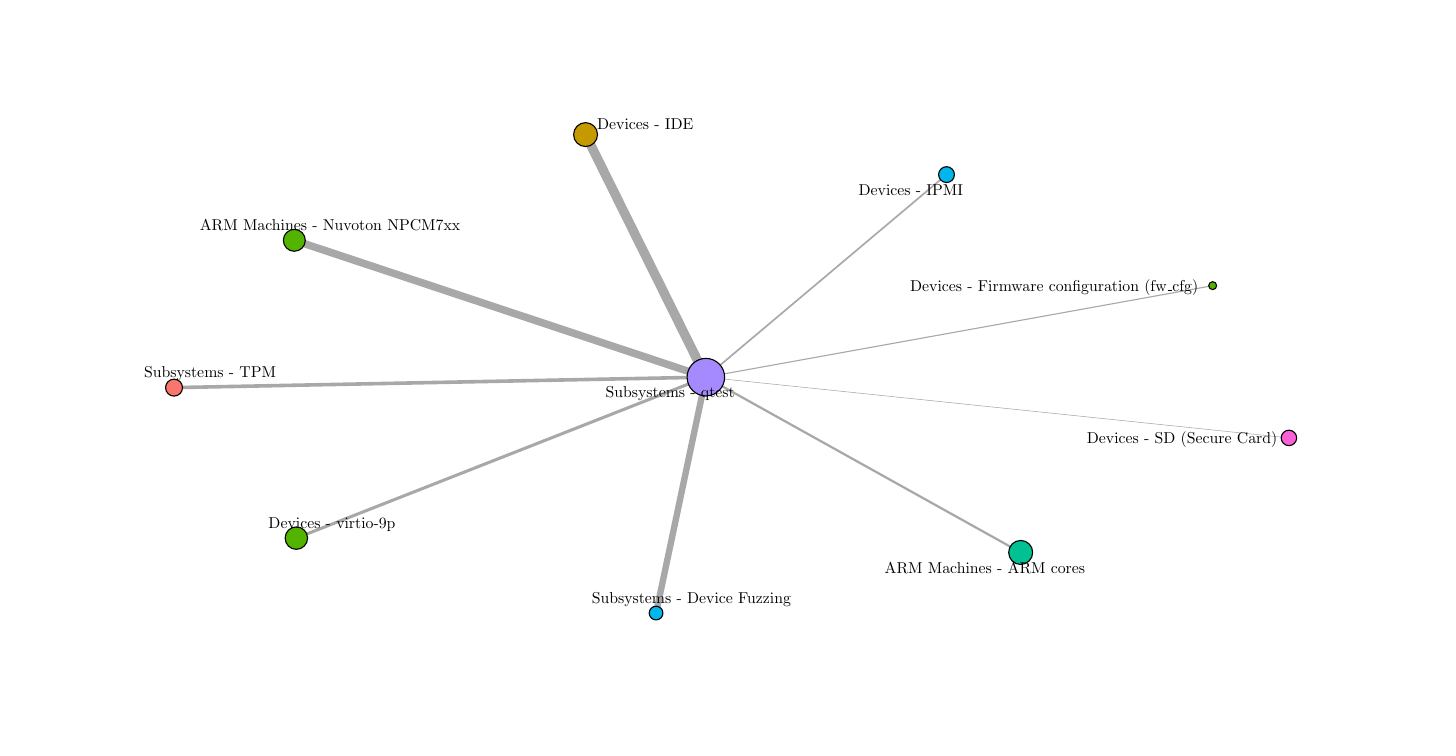
\begin{tikzpicture}[x=1pt,y=1pt]
\definecolor{fillColor}{RGB}{255,255,255}
\path[use as bounding box,fill=fillColor,fill opacity=0.00] (0,0) rectangle (505.89,252.94);
\begin{scope}
\path[clip] (  0.00,  0.00) rectangle (505.89,252.94);
\definecolor{fillColor}{RGB}{255,255,255}

\path[fill=fillColor] (  0.00,  0.00) rectangle (505.89,252.94);
\end{scope}
\begin{scope}
\path[clip] ( 32.75, 32.75) rectangle (475.89,222.94);
\definecolor{drawColor}{gray}{0.66}

\path[draw=drawColor,line width= 0.8pt,line join=round] (358.82, 63.31) -- (245.06,126.65);

\path[draw=drawColor,line width= 2.7pt,line join=round] ( 96.35,176.10) -- (245.06,126.65);

\path[draw=drawColor,line width= 0.4pt,line join=round] (428.19,159.71) -- (245.06,126.65);

\path[draw=drawColor,line width= 3.4pt,line join=round] (201.59,214.30) -- (245.06,126.65);

\path[draw=drawColor,line width= 0.6pt,line join=round] (332.02,199.84) -- (245.06,126.65);

\path[draw=drawColor,line width= 0.2pt,line join=round] (455.75,104.70) -- (245.06,126.65);

\path[draw=drawColor,line width= 1.1pt,line join=round] ( 97.09, 68.49) -- (245.06,126.65);

\path[draw=drawColor,line width= 2.3pt,line join=round] (227.07, 41.40) -- (245.06,126.65);

\path[draw=drawColor,line width= 1.3pt,line join=round] ( 52.89,122.87) -- (245.06,126.65);
\definecolor{drawColor}{RGB}{0,0,0}
\definecolor{fillColor}{RGB}{0,192,148}

\path[draw=drawColor,line width= 0.4pt,line join=round,line cap=round,fill=fillColor] (358.82, 63.31) circle (  4.34);
\definecolor{fillColor}{RGB}{83,180,0}

\path[draw=drawColor,line width= 0.4pt,line join=round,line cap=round,fill=fillColor] ( 96.35,176.10) circle (  3.96);

\path[draw=drawColor,line width= 0.4pt,line join=round,line cap=round,fill=fillColor] (428.19,159.71) circle (  1.43);
\definecolor{fillColor}{RGB}{196,154,0}

\path[draw=drawColor,line width= 0.4pt,line join=round,line cap=round,fill=fillColor] (201.59,214.30) circle (  4.32);
\definecolor{fillColor}{RGB}{0,182,235}

\path[draw=drawColor,line width= 0.4pt,line join=round,line cap=round,fill=fillColor] (332.02,199.84) circle (  2.86);
\definecolor{fillColor}{RGB}{251,97,215}

\path[draw=drawColor,line width= 0.4pt,line join=round,line cap=round,fill=fillColor] (455.75,104.70) circle (  2.79);
\definecolor{fillColor}{RGB}{83,180,0}

\path[draw=drawColor,line width= 0.4pt,line join=round,line cap=round,fill=fillColor] ( 97.09, 68.49) circle (  4.05);
\definecolor{fillColor}{RGB}{0,182,235}

\path[draw=drawColor,line width= 0.4pt,line join=round,line cap=round,fill=fillColor] (227.07, 41.40) circle (  2.48);
\definecolor{fillColor}{RGB}{248,118,109}

\path[draw=drawColor,line width= 0.4pt,line join=round,line cap=round,fill=fillColor] ( 52.89,122.87) circle (  3.06);
\definecolor{fillColor}{RGB}{165,138,255}

\path[draw=drawColor,line width= 0.4pt,line join=round,line cap=round,fill=fillColor] (245.06,126.65) circle (  6.78);

\node[text=drawColor,anchor=base,inner sep=0pt, outer sep=0pt, scale=  0.57] at (345.90, 55.83) {ARM Machines - ARM cores};

\node[text=drawColor,anchor=base,inner sep=0pt, outer sep=0pt, scale=  0.57] at (109.26,179.68) {ARM Machines - Nuvoton NPCM7xx};

\node[text=drawColor,anchor=base,inner sep=0pt, outer sep=0pt, scale=  0.57] at (370.93,157.75) {Devices - Firmware configuration (fw{\_{}}cfg)};

\node[text=drawColor,anchor=base,inner sep=0pt, outer sep=0pt, scale=  0.57] at (223.18,216.00) {Devices - IDE};

\node[text=drawColor,anchor=base,inner sep=0pt, outer sep=0pt, scale=  0.57] at (319.14,192.34) {Devices - IPMI};

\node[text=drawColor,anchor=base,inner sep=0pt, outer sep=0pt, scale=  0.57] at (417.14,102.66) {Devices - SD (Secure Card)};

\node[text=drawColor,anchor=base,inner sep=0pt, outer sep=0pt, scale=  0.57] at (109.96, 72.06) {Devices - virtio-9p};

\node[text=drawColor,anchor=base,inner sep=0pt, outer sep=0pt, scale=  0.57] at (239.83, 44.93) {Subsystems - Device Fuzzing};

\node[text=drawColor,anchor=base,inner sep=0pt, outer sep=0pt, scale=  0.57] at ( 65.89,126.45) {Subsystems - TPM};

\node[text=drawColor,anchor=base,inner sep=0pt, outer sep=0pt, scale=  0.57] at (232.19,119.18) {Subsystems - qtest};
\end{scope}
\end{tikzpicture}
